\chapter{Problemløsning}
\section{Metode}
I det følgende beskrives de metoder og processer der er brugt til at udvikle softwaren. Til softwareudvikling er der taget udgangspunkt i metoden Unified Process (UP). Objektorienteret programmering vil desuden kort blive introduceret, da det anvendte programmeringssprog til den ønskede app, vil være objektorienteret. Til dokumentation af det designede software, er der taget udgangspunkt i Unified Modeling Language (UML), der er standard til at modellere objektorienteret programmering. I afsnittet løsningsstrategi vil der blive opstillet en konkret plan for den videre analyse og softwareudvikling.

\subsection{Unified Process (UP)}
UP er en objektorienteret softwareudviklingsproces. Det er en iterativ metode og beskriver en situation, hvor projektet brydes ned til mindre subprojekter (iterationer). Dette gør fremgangsmåden lettere at håndtere og udføre succesfuldt. Hver iteration giver systemet funktionalitet, og når iterationen giver en udvidelse af det færdige system, betegnes denne inkrementel. På denne måde bygges softwaren trinvist op og vil i sidste ende føre til et fuldt funktionelt system. Ved at bryde projektet ned i en serie af iterationer, tillader det en fleksibel tilgang til projektplanlægningen sammenlignet med den gamle vandfaldsmodel som er udformet i mere strikse sekvenser. Hver iteration vil normalt handle om fuldstændig udvikling af en eller flere use-cases. Et andet karakteristika ved UP er, at det er arkitekturcentreret. Dette henviser til hvordan systemet brydes ned i komponenter, og hvordan disse komponenter interagerer og implementeres.\citep{Arlow2002}
 %UP fokuserer desuden på at identificere risici tidligt, hvorved det bliver muligt at identificere hvilke use-cases, det vil være optimalt at koncentrere sig om i starten. Risici er alt hvad der forhindrer succes af projektet. 
\subsubsection{Iterationer}
Hver iteration indeholder alle elementer i et almindeligt softwareudviklingsprojekt: planlægning, analyse og design, konstruktion, integration og test samt en intern eller ekstern udgivelse. For hver iteration findes fem kerneelementer \citep{Arlow2002}:
\begin{itemize}
    \item Krav - Hvad skal systemet kunne?
    \item Analyse - Raffinere og strukturere krav
    \item Design - Realisere krav i et system arkitektur
    \item Implementering - Bygge softwaren
    \item Test - Verificere at implementering virker som ønsket 
\end{itemize}

\subsubsection{Struktur}
UP er overordnet delt ind i fire faser. Hver fase kan have en eller flere iterationer, og for hver iteration udføres de fem kerneelementer. Mængden af arbejde der lægges i de fem kerneelementer, ændres i de forskellige faser i takt med at projektet skrider frem, se figur \ref{fig:UP}. \citep{Arlow2002}
\begin{itemize}
    \item \textbf{Forberedelse}: De grundlæggende visioner for systemet og et overblik over kravene fastslås. Desuden identificeres risici og formål defineres. 
    \item \textbf{Etablering}: Der fastlægges en grundlæggende arkitektur. Systembeskrivelse og kravspecifikationer defineres. Fokus i etableringsfasen er på krav-, analyse- og designelementerne. I slutningen af denne fase bliver implementering et vigtigt element, når den grundlæggende arkitektur er produceret.  
    \item \textbf{Konstruktion}: Systemets funktioner udvikles og testes. Målet er at færdiggøre alle krav, analyse og design og udvikle det endelig system. I denne fase vægtes implementeringselementet. 
    \item \textbf{Overdragelse}: Overgangen hvor systemet leveres til slutbrugeren. 
\end{itemize}

\begin{figure}[H]
\centering
  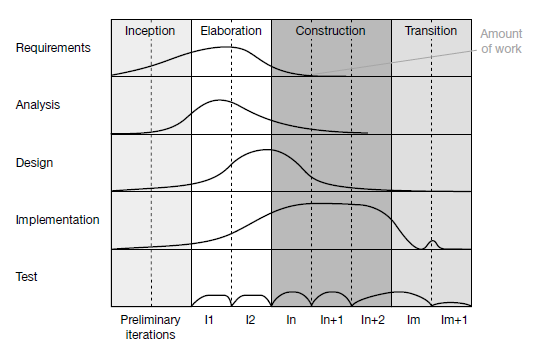
\includegraphics[width=0.8\textwidth]{Billeder/UP.png}
   \caption{Kolonnerne i figuren repræsenterer faserne mens rækkerne repræsenterer de fem kerneelementer. Figuren illustrerer hvordan arbejdsfordeling af de fem kerneelementer varierer afhængig af hvilken fase man befinder sig i. \cite{Arlow2002}} 
   \label{fig:UP}
\end{figure}

\subsection{Objektorienteret programmering}
Ifølge International Data Corporation (IDC), der er et firma der specialiserer sig i markedsanalyser, er Android det mest brugte styresystem til smartphones globalt, med en markedsandel på 85 \% i første kvartal af 2017 \citep{AndroidMarketShare}. I dette projekt programmeres den ønskede app til Android, da dette vil nå flest mennesker. Android er desuden open-source, hvilket vil sige at alle kan programmere apps til Android-styresystemet uden begrænsninger, og gør det muligt simpelt at tilgå hardware i telefonen såsom accelerometer \citep{Meier2010}. Android applikationer er skrevet i programmeringssproget JAVA, der er et objektorienteret sprog \citep{Meier2010}, der her vil blive introduceret.\\
\\
Objektorienteret programmering er et paradigme indenfor softwareudvikling. Den overordnede filosofi er at definere et softwaresystem bestående af en samling af objekter som interagerer med hinanden. Programmeringskoden opdeles i klasser, som hver har sit ansvarsområde i programmet. Et objekt er en instans af en klasse og en klasse kan således genbruges adskillige gange til at skabe objekterne. Klassen er en skabelon som definerer objektets adfærd og består overordnet af to delelementer: attributter og metoder. Attributter definerer objektets egenskaber mens metoder definerer de mulige funktioner som objektet kan udføre. \citep{Dathan}

%Der findes tre grundprincipper i objektorienteret programmering; indkapsling, nedarving og polymorfi. Et objekt indkapsler nogle data og noget funktionalitet (adfærd). Nedarving. Et objekt kan arve data og funktionalitet fra et andet objekt og udvide med med ekstra data og funktionalitet. Polymorfi. To klasser han kave samme grænseflade defineret via nedarving, men udføre dem forskelligt. Java er et eksempel på et almindeligt objektorienteret sprog og systemet er opbygget af indbyrdes sammemhængende objekter. Der er altid et overordnet objekt som instantierer et andet objekt, dvs. laer sin egen kopi af et andet objekt. 

\subsection{Unified Modeling Language (UML)}\label{UML}
UML er et visuelt modelleringssprog, der kan bruges til at beskrive objektorienteret software \citep{Arlow2002}. UML gør det muligt at præsentere de meget varierende aspekter af et softwaresystem som krav, datastruktur, dataflow og informationsflow, ved at bruge objektorienterede koncepter \citep{Seidl2012}. I nuværende version af UML er der 14 forskellige diagrammer, der overordnet kan inddeles i strukturdiagrammer og adfærdsdiagrammer \citep{Seidl2012}. Tages der udgangspunkt i UP, kan arbejdet med UML også deles op i krav, analyse, design og implementering \citep{Arlow2002}. 

\textbf{Krav}\\
Før analyse og design påbegyndes, er der behov for at kravspecifikationerne defineres. Krav danner basis for systemet og fortæller hvad systemet skal kunne gøre \citep{Arlow2002}. I UML bruges use-case-diagrammer til dette, og beskriver hvilke brugere, der bruger hvilke funktionaliteter i systemet \citep{Seidl2012}.

%Der findes to typer af krav: de funktionelle kravspecifikationer som udledes ud fa use-cases og non-funktionelle krav som omhandler begrænsninger af systemet.

\textbf{Analyse}\\
Under analyse skabes modeller der fortæller om systemets ønskede adfærd. Disse modeller fokuserer på, hvad systemet skal kunne gøre, mens hvordan det skal gøre det, defineres under design. \citep{Arlow2002}\\
Aktivitetsdiagrammer er adfærdsdiagrammer, der modellerer en proces som en samling af aktiviteter og overgange mellem aktiviteterne. Bl.a. kan adfærden af use cases beskrives med aktivitetsdiagrammer. \citep{Arlow2002}\\
Under analyse skal relevante analyseklasser desuden defineres. Dette kan gøres ved først at lave en substantiv/verbum-analyse over systembeskrivelsen. \citep{Arlow2002}

\textbf{Design}\\
Formålet med modellering i designfasen, er at specificere hvordan systemets ønskede adfærd opnås \citep{Arlow2002}. Sekvensdiagrammer beskriver interaktionerne mellem objekter der udfører en bestemt handling. Fokus er på den kronologiske orden af beskeder udvekslet mellem interaktionsparterne. \citep{Seidl2012}\\
Designklasser skal desuden defineres ud fra analyseklasserne i analysefasen. Disse er en konkretisering af analyseklasserne, og nogle gange kan det være nødvendigt at dele klasserne op i flere klasser, for at undgå for stor kompleksitet i en enkelt klasse. \citep{Arlow2002}

\textbf{Implementering}\\
Under implementering omsættes de forskellige UML-diagrammer til kode. \citep{Arlow2002}

%\textbf{Use case} Først defineres aktører som direkte interagerer med systemet og findes eksternt for systemet. Derefter opstilles use cases som er noget en aktør ønsker systemet skal kunne gøre. 

%\textbf{Analyse} Skabe modeller som fortæller om systemets ønskede adfærd. Producer analyse modeller som fokuserer på hvad systemet skal kunne gøre mens hvordan det skal gøres overlades til design. 

%Use case realizations: samarbejdet mellem objekter som viser hvordan integaktion mellem objekter kan realiserer en adfærd udtrykt i use cases. 

%Find klasser til objekterne. Klasser består af et sæt af attributer. 

%Problem domænet: domæne hvori brugen for et software system opstår. 

%\begin{itemize}
    %\item Krav: Brugere samt deres behov, hvorudfra der opstilles krav til systemet. Der udarbejdes use cases. Funktionelle og ikke funktionelle krav. 
    %\item Analyse: aktivitivitetsdiagrammer for hver use case med forbindelseselementer. Analyseklasse; hvad skal den kunne men ikke hvordan. Analysediagram: hver klasse samt dens egenskab og relation til hinanden. 
    %\item Design: Specificer hvordan funktionaliteten kan implementeres. Sekvensdiagrammer; hvordan og hvornår i koden forskellige use cases skal benyttes for at opnå den ønskede funktionalitet. 
    %\item Implementering: kodning af de designede modeller. Java. 
    %\item Test: test softwarens funktionalitet; white box og black box test. 
%\end{itemize}

%Brugergrænseflade designprincipper > GUI

\section{Løsningsstrategi}
Softwareudviklingen i dette projekt deles op i fem faser: krav, analyse, design, implementering og test. Under hver fase udarbejdes UML-diagrammer, som beskrevet under afsnit \ref{UML}. Her følger en oversigt over softwareudviklingen.

\begin{enumerate}
    \item Krav
        \begin{itemize}
            \item Systembeskrivelse: Overordnet beskrivelse af systemet og hvad det skal kunne.
            \item Use cases: Identificerer hvilke brugere, der bruger hvilke dele af systemet.
            \item Funktionelle krav: Opstilles på baggrund af use cases.
            \item Non-funktionelle krav: Hvilke begrænsninger systemet har.
        \end{itemize}
    \item Analyse
        \begin{itemize}
            \item Aktivitetsdiagrammer: Adfærden af de opstillede use cases analyseres med aktivitetsdiagrammer.
            \item Substantiv/verbum-analyse: Laves over systembeskrivelsen for at identificere relevante analyseklasser.
            \item Analyseklassediagrammer: Diagrammer over de identificerede klasser fra substantiv/verbum-analysen. I denne fase beskrives klasserne overordnet og abstrakt.
            \item Brugervenlighed: Analyse af hvad brugervenlighed er, og hvordan det skal tænkes ind i systemet.
        \end{itemize}
    \item Design
        \begin{itemize}
            \item Sekvensdiagrammer: Beskriver interaktionen mellem objekter i kronologisk orden.
            \item Designklassediagrammer: Klassediagrammerne fra analysefasen konkretiseres og uddybes.
            \item Brugergrænseflade
        \end{itemize}
    \item Implementering
    \item Test
        \begin{itemize}
            \item Test af funktionelle krav.
            \item Test af non-funktionelle krav.
            \item Opsamling af resultater.
        \end{itemize}
\end{enumerate}
